\documentclass[svgnames]{beamer}
\mode<presentation>
\usefonttheme{serif}
\usecolortheme{dove}
\useinnertheme{rounded}
%\useoutertheme{smoothbars}
\setbeamercolor{item projected}{fg=black}
\setbeamertemplate{navigation symbols}{}

\usepackage[english]{babel}
\usepackage[latin1]{inputenc}
\usepackage{times}
\usepackage{amsthm,amssymb,amsmath,graphicx}
\usepackage{color}
\usepackage{gastex}
\usepackage{framed}
\usepackage{graphicx}
\usepackage{multicol}
\usepackage{ulem}
\usepackage{ifthen}
\usepackage{tikz}
\usetikzlibrary{arrows,positioning} 

%%%%%%%%%%%%%%%%%%%%%%%%%%%%%%%%%%%%%%%%%%%%%%%%%%%%%%%%%%%%%%%%%%%%%%%%%%%%%%%%%%%%%%%%
%%%%%%%%%%%%%%%%%%%% A non-original creation by Nathanaël Fijalkow and Victor Marsault %

\setbeamertemplate{frametitle}{
  \vskip-2pt
  \begin{beamercolorbox}[rightskip=2cm,leftskip=1em,dp=1ex,wd=12.8cm]{frametitle}
    \vskip2pt
    \usebeamercolor{frametitle}
    \begin{tikzpicture}
      \useasboundingbox (0,0) rectangle (0,0); 
      \ifthenelse{\insertframenumber<\inserttotalframenumber}
      { 
        \pgfmathsetmacro{\aimangle}{90-(\insertframenumber*360/\inserttotalframenumber)}
        \fill [fill=frametitle.fg,thin, color=gray!50,draw=black] (11.8,.2) -- (11.8,.6) arc (90:\aimangle:0.4) -- cycle;

      }{ 
        \fill[fill=frametitle.fg,thin, color=gray!50,draw=black] (11.8,0.2) circle (.4);
      }
      \fill[fill=frametitle.fg,thin, color=white,draw=black] (11.8,0.2) circle (.3);
      \node at (11.8, .2) [black,circle]{\normalsize\insertframenumber};
    \end{tikzpicture}
    \insertframetitle
    \vskip2pt
  \end{beamercolorbox}
}
%%%%%%%%%%%%%%%%%%%%%%%%%%%%%%%%%%%%%%%%%%%%%%%%%%%%%%%%%%%%%%%%%%%%%%%%%%%%%%%%%%%%%%%

\setbeamertemplate{blocks}[rounded]
\setbeamercolor{block title}{bg=normal text.bg!90!black}
\setbeamercolor{block body}{bg=normal text.bg!95!black}

\renewcommand{\AA}{\mathcal{A}}

\newcommand{\PSPACE}{\mathrm{PSPACE}}
\newcommand{\BB}{\mathcal{B}}
\newcommand{\CC}{\mathcal{C}}
\newcommand{\JJ}{\mathcal{J}}
\newcommand{\DD}{\mathcal{D}}
\newcommand{\KK}{\mathcal{K}}
\newcommand{\LL}{\mathcal{L}}
\newcommand{\HH}{\mathcal{H}}
\newcommand{\GG}{\mathcal{G}}
\newcommand{\RR}{\mathbb{R}}
\newcommand{\NN}{\mathbb{N}}
\newcommand{\QQ}{\mathbb{Q}}
\newcommand{\MM}{\mathcal{M}}
\newcommand{\MMAA}{\MM_\AA}
\newcommand{\tr}[1]{\langle #1 \rangle}
\newcommand{\prob}[1]{\mathbb{P}_{#1}}
\newcommand{\stab}[1]{S(#1)}
\newcommand{\set}[1]{\{ #1 \}}
\newcommand{\val}[1]{\text{val}(#1)}

\newcommand{\ProA}{\widehat{A^*}}
\newcommand{\ProProA}{\widetilde{A^*}}
\newcommand{\PPA}[1]{\ProProA[#1]}

\renewcommand{\P}{\mathbb{P}}

\newtheorem{conjecture}{Conjecture}
  
\title{The Value $1$ Problem\\
for Probabilistic Automata}
\author{Nathana\"el Fijalkow}
\institute{LIAFA, Universit\'e Denis Diderot - Paris 7, France\\
Institute of Informatics, Warsaw University, Poland\\
\textbf{nath@liafa.univ-paris-diderot.fr}}

\date{September 4th, 2014}

\AtBeginSection[]
{
\addtocounter{framenumber}{-1}
  \begin{frame}<beamer>{Outline}
    \tableofcontents[currentsection]
  \end{frame}
}

\AtBeginSubsection[]
{
\addtocounter{framenumber}{-1}
  \begin{frame}<beamer>{Outline}
    \tableofcontents[currentsection,currentsubsection]
  \end{frame}
}

\begin{document}

\addtocounter{framenumber}{-1}

\begin{frame}
  \titlepage
\end{frame}

\begin{frame}{A Real-life Situation}
\only<1>{
\begin{center}
\begin{picture}(100,50)(0,0)
	\gasset{Nadjust=wh,Nadjustdist=2,fillcolor=Gray!50}

  	\node[Nmarks=i,iangle=235](H1)(0,30){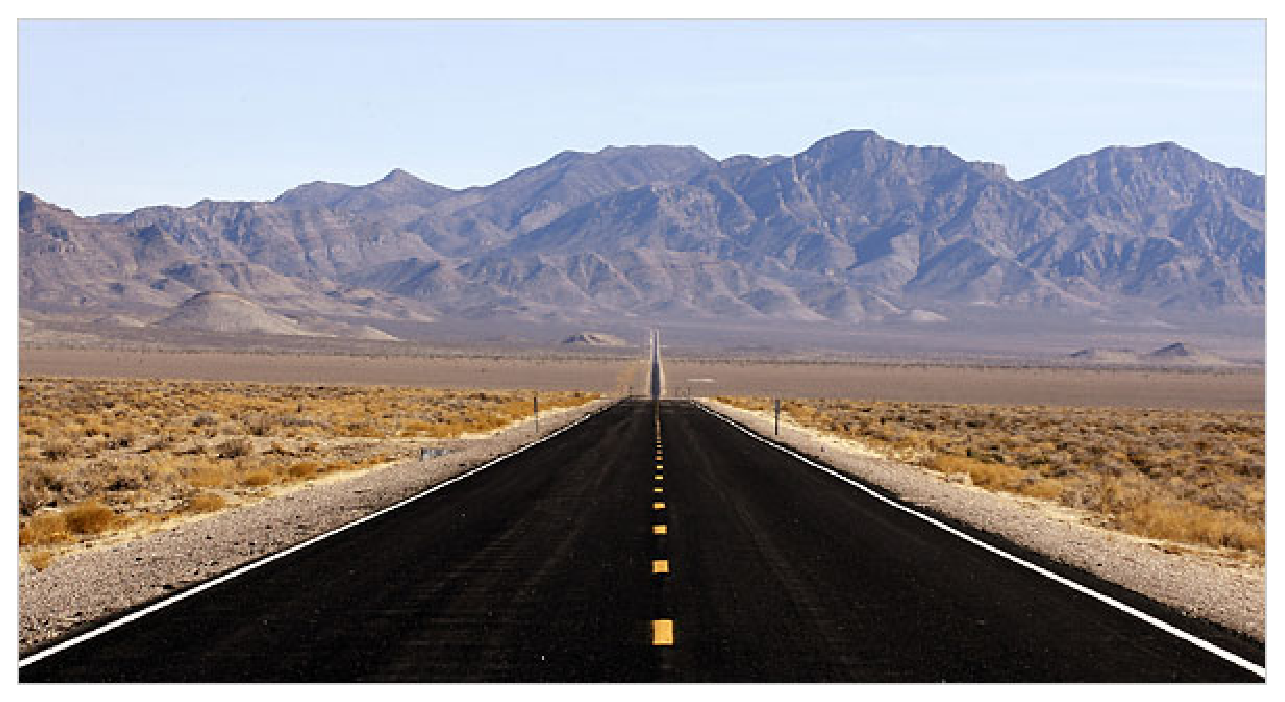
\includegraphics[scale=.1]{high.eps}}
  	\node[linecolor=White](H1)(0,30){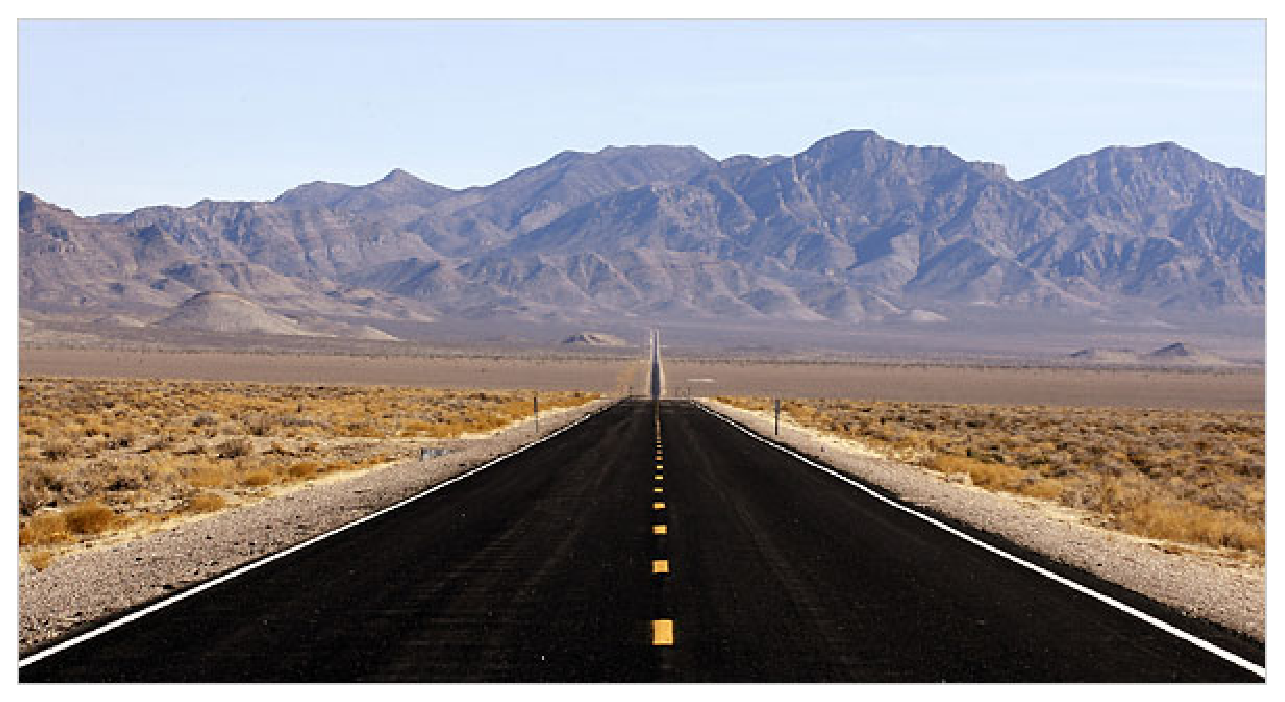
\includegraphics[scale=.1]{high.eps}}
  	\node[linecolor=White](H2)(50,30){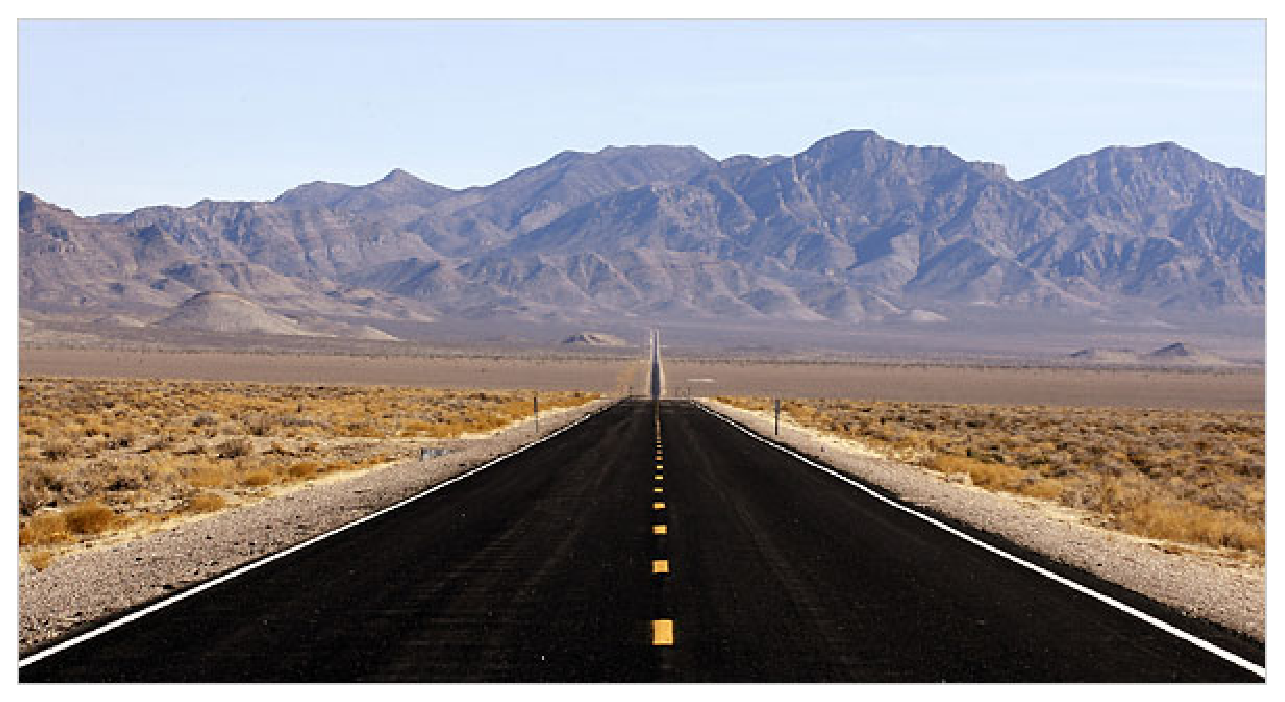
\includegraphics[scale=.1]{high.eps}}
  	\node[linecolor=White](H3)(100,30){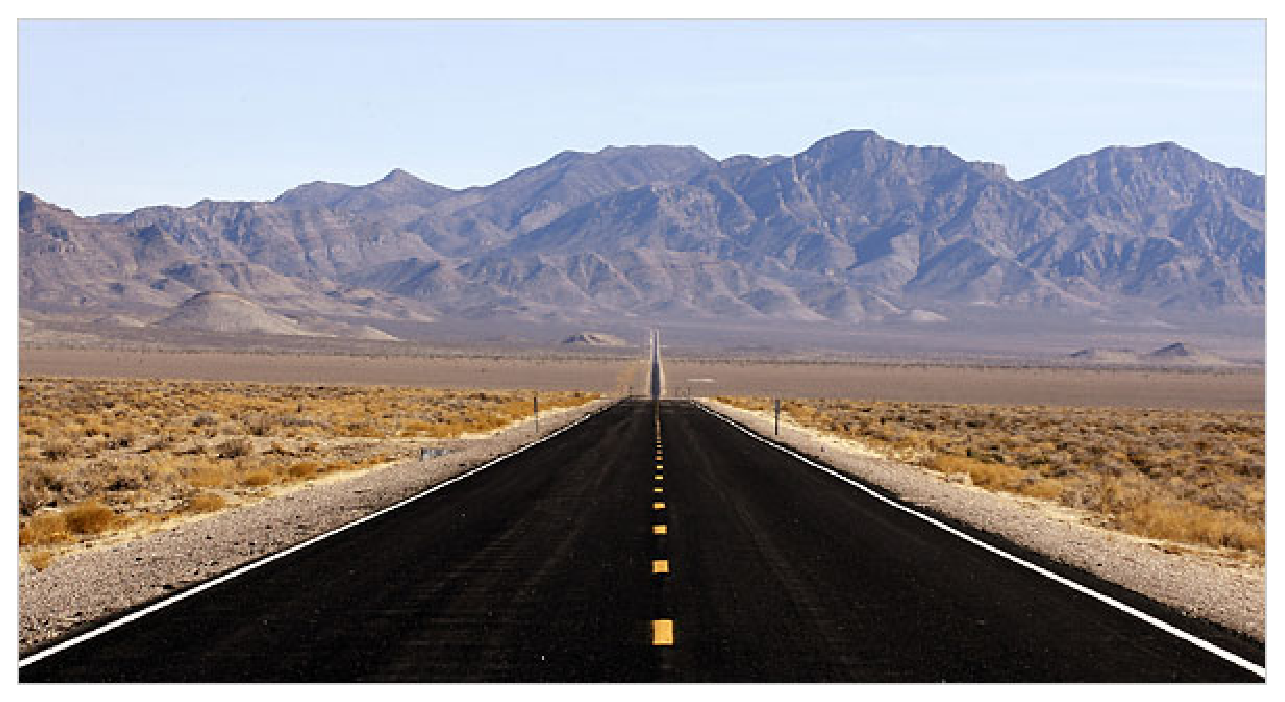
\includegraphics[scale=.1]{high.eps}}
  	\node[linecolor=White](N)(25,0){
\includegraphics[scale=.18]{lost.eps}}
  	\node[linecolor=White](C)(75,0){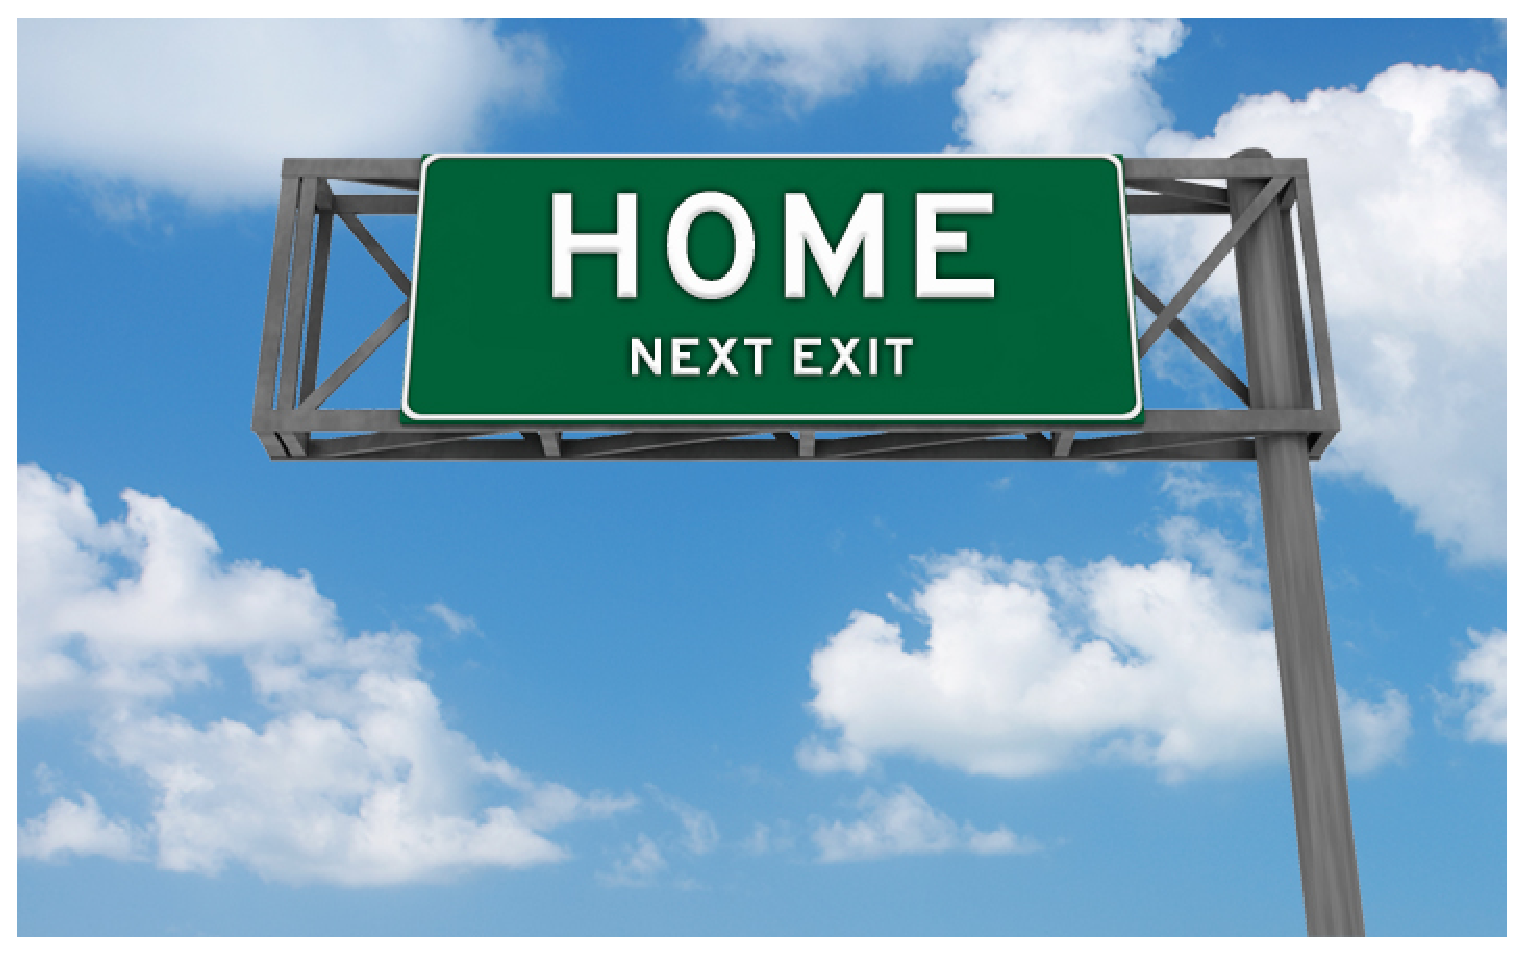
\includegraphics[scale=.1]{home.eps}}

  	\drawedge(H1,H2){$\textrm{drive}:0.6$}
  	\drawedge(H2,H3){$\textrm{drive}:0.55$}
  	\drawedge[curvedepth=-30](H3,H1){$\textrm{exit}$}
	\drawloop[loopangle=90](H1){$\textrm{drive}:0.4$}
	\drawloop[loopangle=90](H2){$\textrm{drive}:0.45$}
	\drawloop[loopangle=90](H3){$\textrm{drive}$}
  	\drawedge[curvedepth=-5](H1,N){$\textrm{exit}$}
  	\drawedge[curvedepth=-5](H2,C){$\textrm{exit}$}
	\drawloop[loopangle=180](N){}
	\drawloop[loopangle=180](C){}
\end{picture}
\end{center}
}
\only<2>{
\begin{columns}[t]
\begin{column}{0.5\textwidth}
\begin{center}
\scalebox{.5}{
\begin{picture}(100,50)(0,0)
	\gasset{Nadjust=wh,Nadjustdist=2,fillcolor=Gray!50}

  	\node[Nmarks=i,iangle=235](H1)(0,30){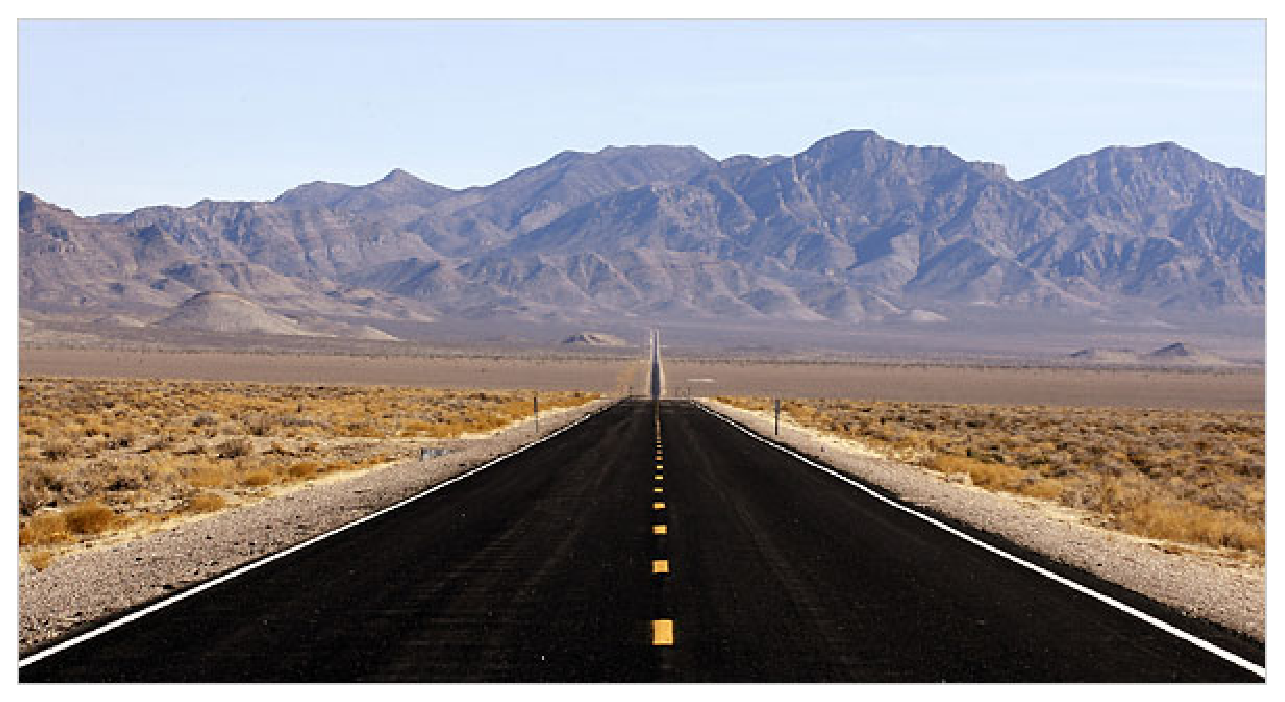
\includegraphics[scale=.1]{high.eps}}
  	\node[linecolor=White](H1)(0,30){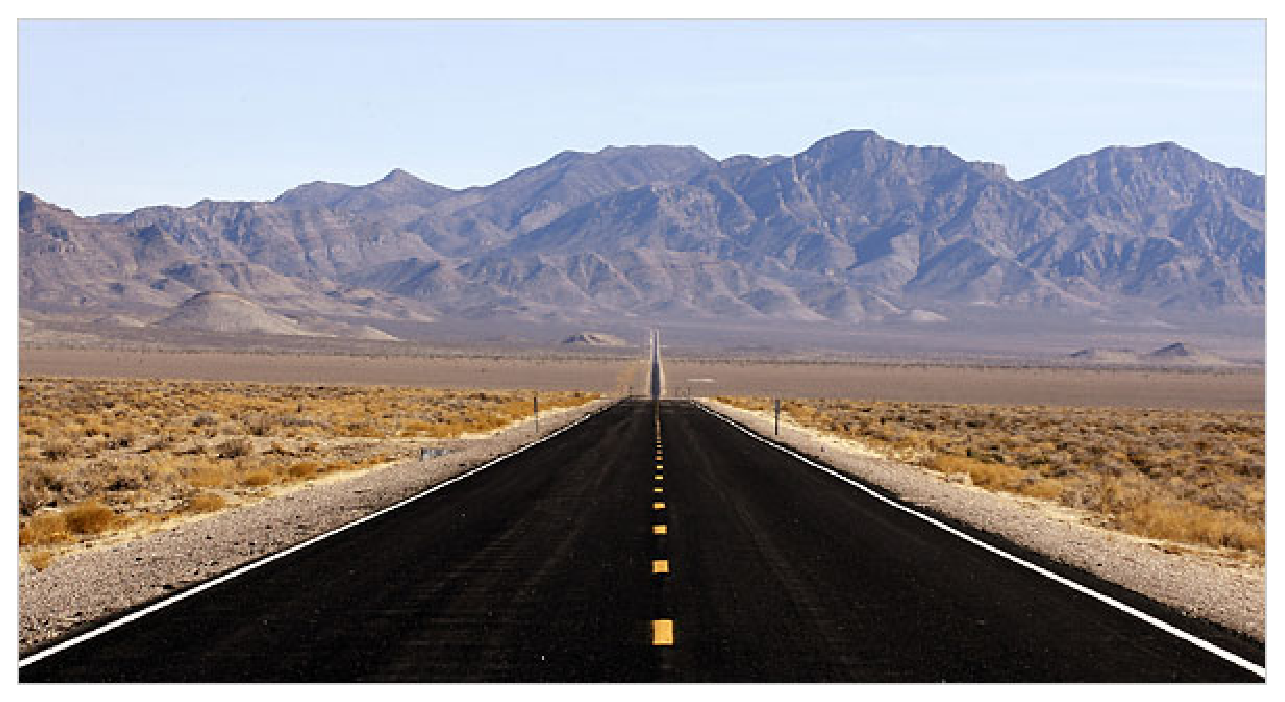
\includegraphics[scale=.1]{high.eps}}
  	\node[linecolor=White](H2)(50,30){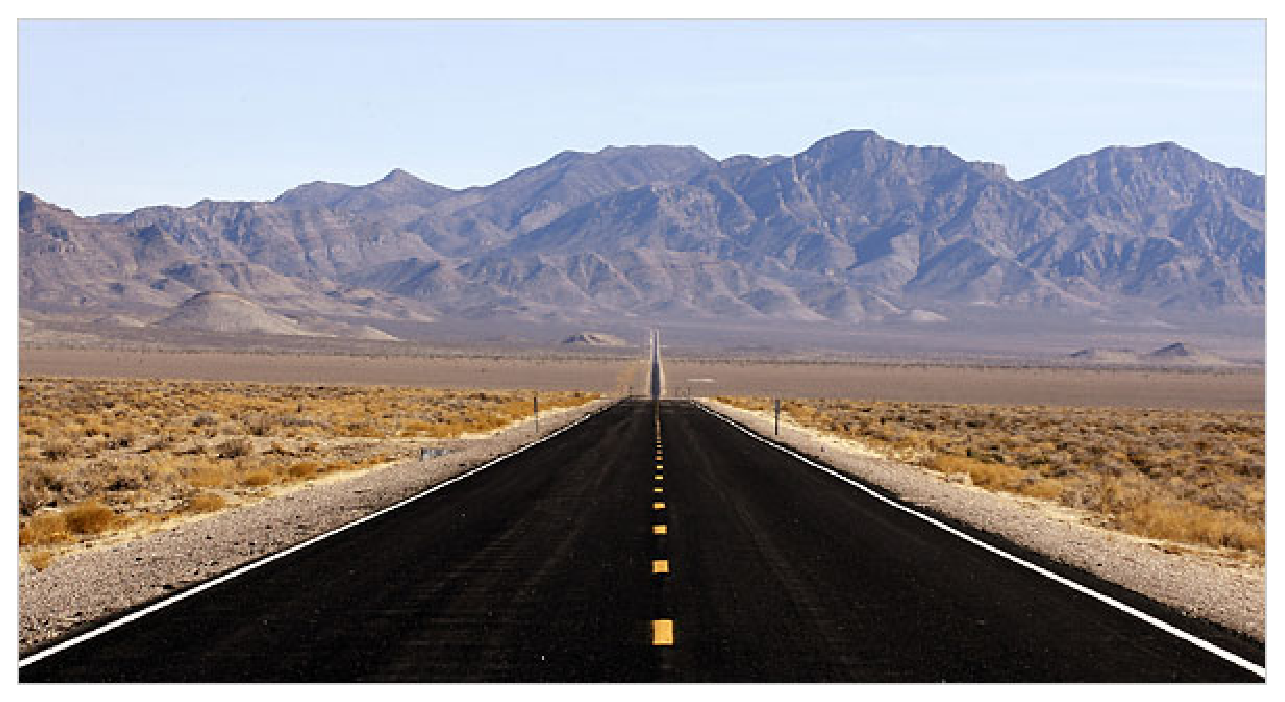
\includegraphics[scale=.1]{high.eps}}
  	\node[linecolor=White](H3)(100,30){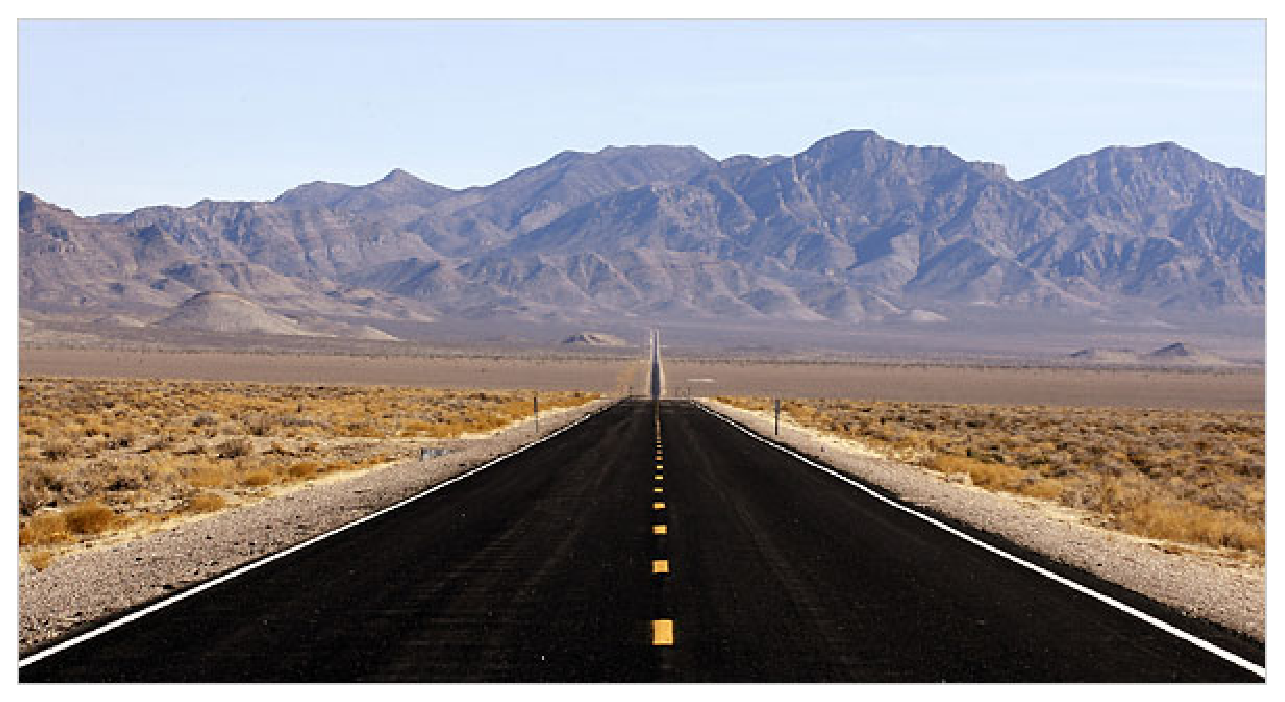
\includegraphics[scale=.1]{high.eps}}
  	\node[linecolor=White](N)(25,0){
\includegraphics[scale=.18]{lost.eps}}
  	\node[linecolor=White](C)(75,0){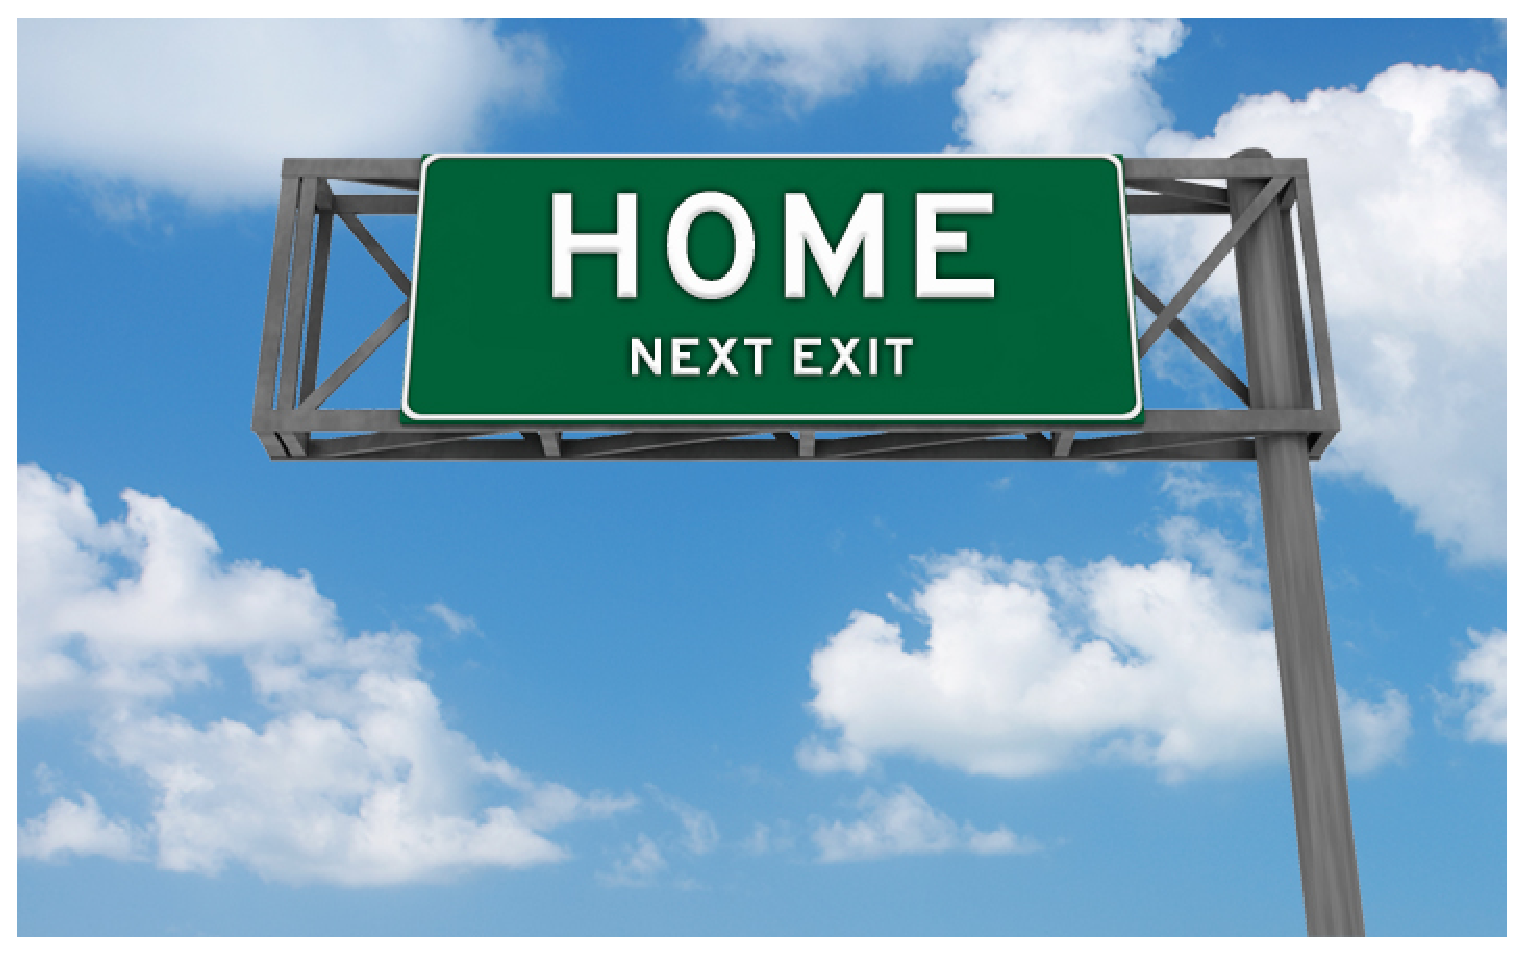
\includegraphics[scale=.1]{home.eps}}

  	\drawedge(H1,H2){$\textrm{drive}:0.6$}
  	\drawedge(H2,H3){$\textrm{drive}:0.55$}
  	\drawedge[curvedepth=-30](H3,H1){$\textrm{exit}$}
	\drawloop[loopangle=90](H1){$\textrm{drive}:0.4$}
	\drawloop[loopangle=90](H2){$\textrm{drive}:0.45$}
	\drawloop[loopangle=90](H3){$\textrm{drive}$}
  	\drawedge[curvedepth=-5](H1,N){$\textrm{exit}$}
  	\drawedge[curvedepth=-5](H2,C){$\textrm{exit}$}
	\drawloop[loopangle=180](N){}
	\drawloop[loopangle=180](C){}
\end{picture}
}
\end{center}
\end{column}
\begin{column}{0.5\textwidth}
\begin{itemize}
	\item No sequence of actions ensure to reach home \textcolor{red}{\textit{almost surely}}.
	\item For every $\varepsilon > 0$, there exists a sequence of actions ensuring to reach home
with probability at least $1 - \varepsilon$!
	\item This is not true anymore if the probabilities change!
\end{itemize}
\end{column}
\end{columns}
}
\end{frame}

\begin{frame}{The Value 1 Problem}

\begin{columns}[t]
\begin{column}{0.5\textwidth}
\begin{figure}
\begin{center}
\begin{picture}(20,40)(0,-10)
	\gasset{Nw=6,Nh=6,fillcolor=Gray!50}

  	\node[linecolor=White,Nmarks=i,iangle=0](L1)(15,15){$1$}
  	\node[linecolor=White](L2)(0,30){$2$}
  	\node[linecolor=White,Nmarks=r](L3)(0,0){$3$}

  	\drawedge(L1,L2){$b$}
  	\drawedge[curvedepth=-5,ELside=r](L1,L3){$a:0.4$}
  	\drawedge[curvedepth=-5,ELside=r](L3,L1){$b$}
	\drawloop(L1){$a:0.6$}
	\drawloop[loopangle=135](L2){$a,b$}
	\drawloop[loopangle=215](L3){$a$}
\end{picture}
\end{center}
\end{figure}
\end{column}
\begin{column}{0.5\textwidth}
\vskip1em
$$\prob{\AA} : A^* \rightarrow [0,1]$$
\begin{center}
$\prob{\AA}(w)$ is the probability that a run for $w$ is successful.
\end{center}
\end{column}
\end{columns}

\begin{framed}
INPUT: $\AA$ a probabilistic automaton\\
OUTPUT: for all $\varepsilon > 0$, there exists $w \in A^*$,
$\prob{\AA}(w) \ge 1 - \varepsilon$.
\end{framed}
In other words, define $\val{\AA} = \sup_{w \in A^*} \prob{\AA}(w)$, is $\val{\AA} = 1$?
\end{frame}

\begin{frame}{A Research Program}
Starting point:
\begin{theorem}[Gimbert and Oualhadj, 2010]
The value $1$ problem is undecidable.
\end{theorem}

\begin{center}
\begin{huge}
But \textit{to what extent}?
\end{huge}
\pause
\vskip2em
Construct an algorithm to decide the value $1$ problem,\\
which is \textcolor{red}{\textit{often}} correct.
\vskip2em
\pause
Quantify \textcolor{red}{\textit{how often}}.
\vskip2em
\pause
Argue that you cannot do \textcolor{red}{\textit{more often}} than that.
\end{center}
\end{frame}

\begin{frame}{What was known?}
\begin{columns}[t]
\begin{column}{0.6\textwidth}
\begin{center}
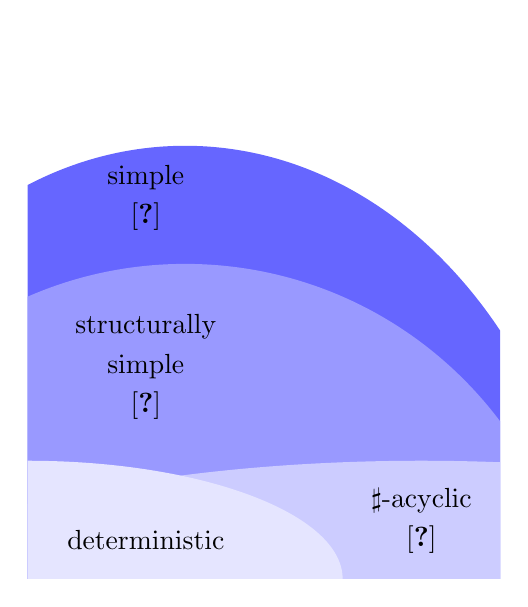
\begin{tikzpicture}
\clip (-6,2) rectangle (0,9);

%\fill[red!90] (-1,5) ellipse (8cm and 4cm) ;
%\draw (-1,8) node {leaktight} ;
%\draw (-1,7.5) node {\cite{FGO12}} ;

\fill[blue!60] (-4,1) ellipse (5.2cm and 6.5cm) ;
\draw (-4.5,7.1) node {simple} ;
\draw (-4.5,6.6) node {\cite{CT12}} ;

\fill[blue!40] (-4,1) ellipse (5cm and 5cm) ;
\draw (-4.5,5.2) node {structurally} ;
\draw (-4.5,4.7) node {simple} ;
\draw (-4.5,4.2) node {\cite{CT12}} ;

\fill[blue!20] (-1,1) ellipse (8cm and 2.5cm) ;
\draw (-1,3) node {$\sharp$-acyclic} ;
\draw (-1,2.5) node {\cite{GO10}} ;

\fill[blue!10] (-6,2) ellipse (4cm and 1.5cm) ;
\draw (-4.5,2.5) node {deterministic} ;
\end{tikzpicture}
\end{center}
\end{column}
\begin{column}{0.52\textwidth}
\vskip5em
\begin{theorem}[\cite{BBG12,CSV13}]
The value $1$ problem is $\Sigma^0_2$-complete.
\end{theorem}
\end{column}
\end{columns}
\end{frame}

\begin{frame}{Our Contributions}
\begin{columns}[t]
\begin{column}{0.6\textwidth}
\begin{center}
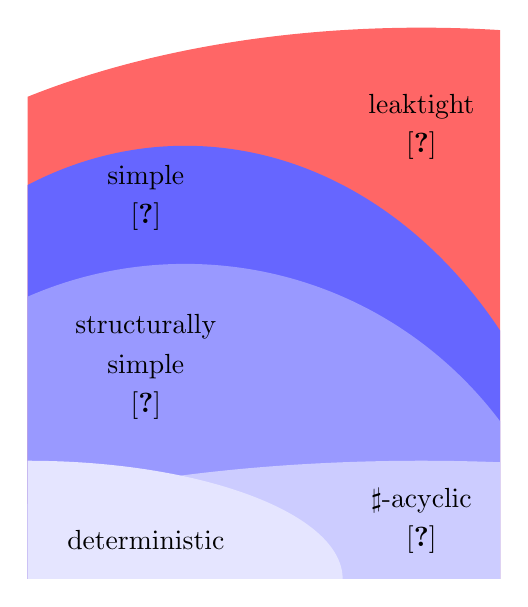
\begin{tikzpicture}
\clip (-6,2) rectangle (0,9);

\fill[red!60] (-1,5) ellipse (8cm and 4cm) ;
\draw (-1,8) node {leaktight} ;
\draw (-1,7.5) node {\cite{FGO12}} ;

\fill[blue!60] (-4,1) ellipse (5.2cm and 6.5cm) ;
\draw (-4.5,7.1) node {simple} ;
\draw (-4.5,6.6) node {\cite{CT12}} ;

\fill[blue!40] (-4,1) ellipse (5cm and 5cm) ;
\draw (-4.5,5.2) node {structurally} ;
\draw (-4.5,4.7) node {simple} ;
\draw (-4.5,4.2) node {\cite{CT12}} ;

\fill[blue!20] (-1,1) ellipse (8cm and 2.5cm) ;
\draw (-1,3) node {$\sharp$-acyclic} ;
\draw (-1,2.5) node {\cite{GO10}} ;

\fill[blue!10] (-6,2) ellipse (4cm and 1.5cm) ;
\draw (-4.5,2.5) node {deterministic} ;
\end{tikzpicture}
\end{center}
\end{column}
\begin{column}{0.5\textwidth}
\pause
In \cite{FGO12},
we introduced the Markov Monoid,
generalizing the transition monoid.
\vskip1em
\begin{theorem}[\cite{FGO12}]
The value $1$ problem is decidable for leaktight automata.
\end{theorem}
\begin{theorem}[\cite{FGKO14}]
Leaktight automata strictly contain the simple automata.
\end{theorem}
\begin{theorem}[\cite{F14}]
\textcolor{red}{The Markov Monoid algorithm is \textit{optimal}.}
\end{theorem}
\end{column}
\end{columns}
\end{frame}

\begin{frame}{Drawing the Decidability Frontier}
\begin{columns}[t]
\begin{column}{0.6\textwidth}
The following are equivalent:
\begin{itemize}
	\item The value $1$ problem over finite words,
	\item The emptiness problem over prostochastic words.
\end{itemize}

\pause
\begin{theorem}[\cite{F14}]\hfill
\begin{enumerate}
	\item The Markov Monoid Algorithm answers ``YES'' if and only if
	there exists a regular $\omega$-term accepted by $\AA$,
	\item The following problem is undecidable: determine whether
	there exists an $\omega$-term on the level $2$ accepted by $\AA$.
\end{enumerate}
\end{theorem}

\end{column}
\begin{column}{0.5\textwidth}
\begin{center}
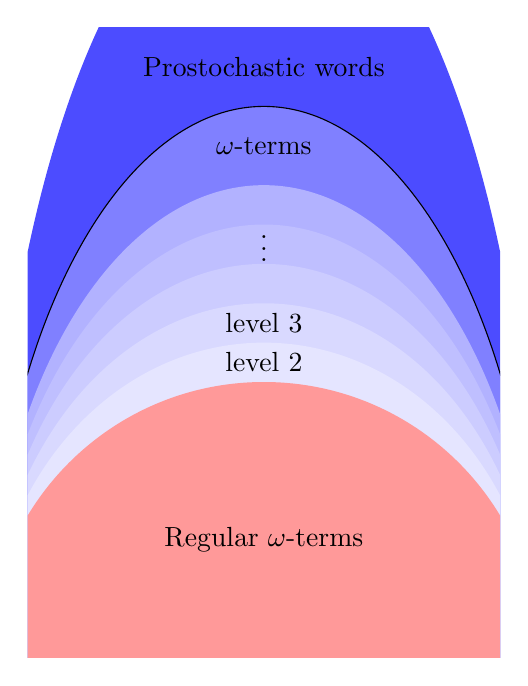
\begin{tikzpicture}
\clip (-3,1) rectangle (3,9);

\fill[blue!70] (0,1) ellipse (3.5cm and 10cm) ;
\draw (0,8.5) node {Prostochastic words} ;

\fill[blue!50] (0,1) ellipse (3.5cm and 7cm) ;
\draw[black] (0,1) ellipse (3.5cm and 7cm) ;
\draw (0,7.5) node {$\omega$-terms} ;
\fill[blue!30] (0,1) ellipse (3.5cm and 6cm) ;
\fill[blue!25] (0,1) ellipse (3.5cm and 5.5cm) ;
\draw (0,6.3) node {$\vdots$} ;
\fill[blue!20] (0,1) ellipse (3.5cm and 5cm) ;
\fill[blue!15] (0,1) ellipse (3.5cm and 4.5cm) ;
\draw (0,5.25) node {level $3$} ;
\fill[blue!10] (0,1) ellipse (3.5cm and 4cm) ;
\draw (0,4.75) node {level $2$} ;
\draw (0,3.75) node {\textcolor{red}{Undecidable}} ;

\fill[red!40] (0,1) ellipse (3.5cm and 3.5cm) ;
\draw (0,2.5) node (reg) {Regular $\omega$-terms} ;
\end{tikzpicture}   
\end{center}
\end{column}
\end{columns}
\end{frame}

\begin{frame}{Conclusion}
\begin{center}
We introduced the Markov Monoid Algorithm\\
to solve the value $1$ problem for leaktight automata~\cite{FGO12}.\\

\pause
\vskip2em

This algorithm is \textit{so far}, the \textit{most correct} algorithm\\
to solve the value $1$ problem~\cite{FGKO14}.\\

\pause
\vskip2em

\textit{In some sense}, this algorithm is optimal~\cite{F14}.

\pause
\vskip2em
\begin{Huge}Thank you!\end{Huge}
\end{center}
\end{frame}

\bibliographystyle{alpha}
\bibliography{bib}

\end{document}
